%------------------------------------------------------------
\documentclass[11pt,a4paper,notitlepage]{article}%
%Options -- Point size:  10pt (default), 11pt, 12pt
%        -- Paper size:  letterpaper (default), a4paper, a5paper, b5paper
%                        legalpaper, executivepaper
%        -- Print size:  oneside (default), twoside

\usepackage{amsmath}						% American Mathematical Society package
\usepackage{amsfonts}
\usepackage{amssymb}
\usepackage{bm}								% bold math
\usepackage{caption}						% caption for figure in minipage
\usepackage[utf8]{inputenc}
\usepackage[slovene]{babel}
\usepackage[style=german]{csquotes}
\usepackage[
	backend=biber,
	style=ieee]{biblatex}
\addbibresource{preamble.bib}
\usepackage{graphicx}							% Define font colors, page xolors, boxes with background color, rotate text in a box, scale text vertically and horizontally, put graphics in a box.

\usepackage{verbatim}							% Za večvrstične komentarje.
\usepackage{setspace}							% Za svobodno spreminjanje razmika med vrsticami.
\usepackage{parskip}
\setlength{\parindent}{0pt}
\usepackage{fancyhdr}
\linespread{1}
\usepackage[font=normalsize]{caption}  		 	% Za poljubno poravnavo imen slik, tabel, itd.
\usepackage{subcaption}
\usepackage[retainorgcmds]{IEEEtrantools}  		% Za lepšo obliko večvrstičnih enačb.
\usepackage[unicode]{hyperref} 					% Za povezave v kazalu.
\hypersetup{
    colorlinks,
    citecolor=black,
    filecolor=black,
    linkcolor=black,
    urlcolor=black
}
\usepackage{url} 								% Za dolge spletne naslove.
\usepackage{placeins} 							% Za FloatBarrier.
\usepackage{booktabs}							% Za TabItem (pikica pri seznamu).
\usepackage{xcolor}								% Required by tabu.
\usepackage{colortbl}							% Required by tabu.
\usepackage{tabu}							% Width-adjustable tabular.
\newcommand{\tabitem}{~~\llap{\textbullet}~~}
%\usepackage{sectsty} % Za veèje naslove.
%\sectionfont{\huge}
%\subsectionfont{\LARGE}


% OKRAJŠAVE MATEMATIČNIH SIMBOLOV

\def\rcurs{{\mbox{$\resizebox{.09in}{.08in}{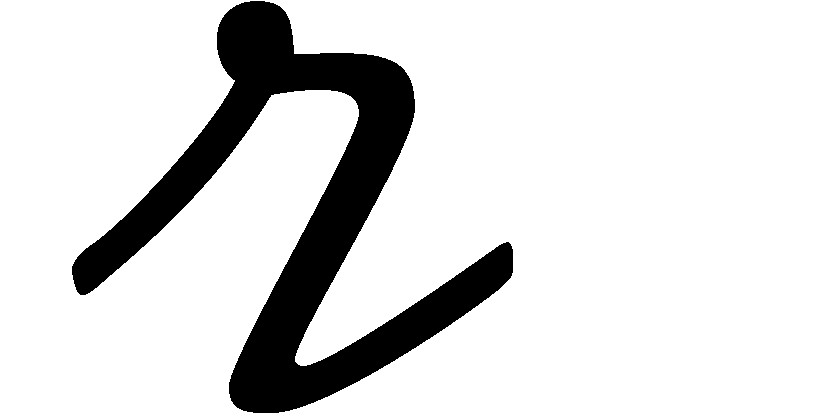
\includegraphics[trim= 1em 0 14em 0,clip]{TeX/ScriptR}}$}}}
\def\brcurs{{\mbox{$\resizebox{.09in}{.08in}{
\includegraphics[trim= 1em 0 14em 0,clip]{TeX/BoldR}}$}}}
\renewcommand{\arraystretch}{1.3} 				% Za razmik med vrsticami tabele.
\newcommand{\ud}{\mathrm{d}} 					% Krajše ime diferenciala.
\newcommand{\uD}{\mathrm{D}}					% Diferencialni operator.
\newcommand{\pd}{\partial}						% Parcialni odvod.
\newcommand{\del}{\bm{\nabla}}					% Nabla.
\newcommand{\mathbsf}[1] {\bm{\mathsf{#1}}}
\renewcommand{\Re}{\operatorname{Re}}		  	% Operator za realni del kompleksnega števila.
\renewcommand{\Im}{\operatorname{Im}} 			% Operator za imaginarni del kompleksnega števila.


% NASTAVITEV RAZMIKA MED BESEDILOM IN ENAČBO

\setlength{\belowdisplayskip}{11pt} 			% Razmik pod enačbo, ko je vrstica polna.
\setlength{\abovedisplayskip}{11pt} 			% Razmik nad enačbo, ko je vrstica polna.
\setlength{\belowdisplayshortskip}{11pt}  		% Razmik pod enačbo, ko vrstica ni polna.
\setlength{\abovedisplayshortskip}{0pt}   		% Razmik nad enačbo, ko vrstica ni polna.


% FancyHdr package settings

\pagestyle{fancy}	% Setting for fancyhdr package. Must occur before length adjustments.

% NASTAVITEV BELIH ROBOV, GLAVE IN NOGE

\setlength{\voffset}{-1.0in}			% Top to Header Top Margin = 1 inch+\voffset
\setlength{\topmargin}{1.0cm}			% Header Top Margin Height
\setlength{\headheight}{1.75cm}
\setlength{\headsep}{0.35cm}			% Header Lower Margin Height
\setlength{\textheight}{24.7cm}			% Header Lower Margin to Footer height
\setlength{\footskip}{1.0cm}

\setlength{\headwidth}{17.0cm}
\setlength{\hoffset}{-1.0in}			% Left page padding = 1 inch + \hoffset
\setlength{\oddsidemargin}{2.0cm}
\setlength{\textwidth}{17.0cm}
\setlength{\marginparsep}{0.0cm}
\setlength{\marginparwidth}{0.0cm}		% Width of "side notes margin."			% 

\fancyhead[L]{
	\large{Marko Petek} \\[0.3cm]
}
\fancyhead[C]{
\includegraphics[height=1.6cm]{Slike/logo-um-fnm}}
\fancyhead[R]{
	\large{Maribor, 19.\ I.\ 2019} \\[0.3cm]
}
\cfoot{\thepage}
\renewcommand{\headrulewidth}{0.0cm}							% Horizontal line in header
\renewcommand{\footrulewidth}{0.0cm}							% Horizontal line in footer


%-------------------------------------------°

\begin{document}

% TITLE PAGE

%	\setlength{\voffset}{-1.7cm}  																																% Set margins.
%	\setlength{\headsep}{0cm}
%	\setlength{\headheight}{0cm}

	\begin{center}
		\textbf{\LARGE{Metoda končnih elementov, ki minimizira kvadrat ostanka aproksimacije}}\\[0.25cm]
		\large{Seminarska naloga pri Naprednih numeričnih metodah}\\[0.7cm]
	\end{center}


% RESET SOME OF THE MARGINS FOR THE REST OF THE DOCUMENT

	%\setlength{\voffset}{-2.15cm}
	%\setlength{\headsep}{0.5cm}
	%\setlength{\headheight}{0.8cm}

%-----------------------------------------------------------------------------%
	
	Numerično reševanje parcialnih diferencialnih enačb (\texttt{PDE}) je zaradi pomanjkanja vsestranskega algoritma še zmeraj bolj umetnost kot ustaljena znanost \cite{JiangB-LSFEM}. Pri zapletenih problemih hitro prispemo do vznožja gore matematične teorije, ki je ni moč zaobiti. Zaradi množice različnih pristopov reševanja ter raztresene in neprijazno napisane literature, lahko le ugibamo, kako visoko se bomo na poti do prelaza morali povzpeti. Zapletenim problemom prostorske dinamike v:
	\begin{center}
		\begin{tabular}[h]{lll}
			\tabitem dinamiki tekočin,\hspace{1cm}	&	\tabitem termodinamiki,\hspace{2.5cm}	&	\tabitem elektrodinamiki,\\
			\tabitem kvantni teoriji,	&	\tabitem splošni teoriji relativnosti,&	\\
		\end{tabular}
	\end{center}
	kjer naletimo na \texttt{PDE}, se tako tudi v višjem izobraževanju najraje izognemo. Metoda končnih elementov (\texttt{FEM}), ki minimizira kvadrat ostanka aproksimacije (\texttt{LSFEM} = Least Squares \texttt{FEM}), obeta razvoj vsestranskega algoritma za reševanje \texttt{PDE} in s tem približanje omenjenih problemov širšemu krogu raziskovalcev.
	
	\section{Temelji FEM}
	Kadar obravnavamo prostorsko dinamiko (npr.\ prevajanje toplote ali tok tekočine), lahko fizični prostor modeliramo kot 1, 2, 3 ali 4-mnogoterost. Temelje \texttt{FEM} bomo polagali na splošnem primeru $d$-mnogoterosti, v prid predstavljivosti pa na njih sproti gradili konkretni 2D primer.
	
	Naj bo prizorišče dogajanja $d$-monogoterost $\Omega$ s krajevnim vektorjem $\mathbf{x}$. Pri reševanju sistema $p$ \texttt{PDE} iščemo p funkcij $u_1(\mathbf{x}), ..., u_p(\mathbf{x})$, ki v vsaki točki odprte domene $\Omega$ zadostijo sistemu \texttt{PDE}, na meji $\Gamma$ pa robnim pogojem. Obravnava bo enostavnejša, če iskane funkcije zložimo v vektor $\mathbf{u}(\mathbf{x})$: \\[0.2cm]
	\begin{tabu} to 1\textwidth {X[1,c]X[1,c]}
		$\mathbf{x} = \begin{bmatrix}
			x_1 \\
			\vdots \\
			x_d \\
		\end{bmatrix} \hspace{1.0cm} d \texttt{ koordinat na }\Omega \ ,$ &
		$\mathbf{u}(\mathbf{x}) = \begin{bmatrix}
			u_1(\mathbf{x}) \\
			\vdots \\
			u_p(\mathbf{x})
		\end{bmatrix} \hspace{1.0cm} p \texttt{ neznank na } \Omega \ .$
	\end{tabu} \\[0.2cm]
	Splošno razlago bomo sproti ilustrirali sistema s tremi spremenljivkami ($p = 3$). \\[0cm]
	
	\begin{minipage}[l]{0.5\textwidth}
		\captionsetup{type=figure}
		\centering
		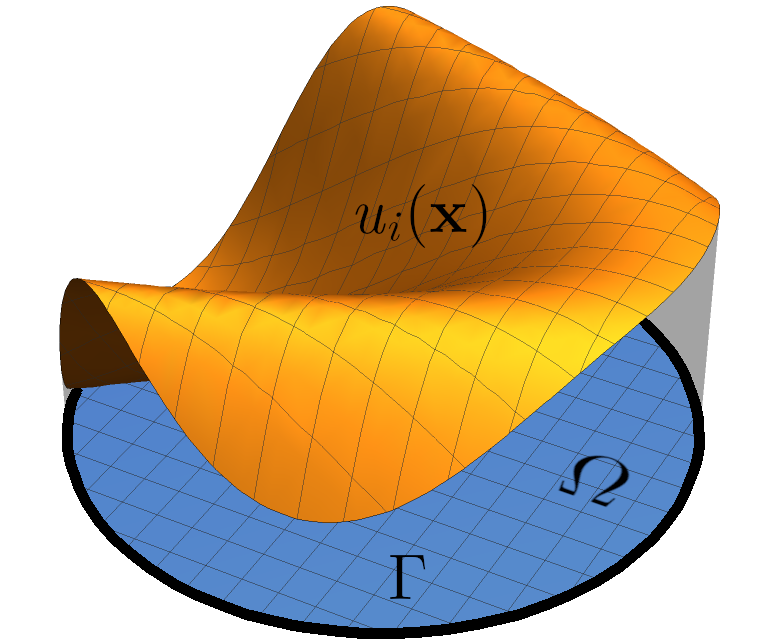
\includegraphics[height=3.7cm]{Slike/funkcijaInDomenaG}
		\caption{Domena $\Omega$, meja domene $\Gamma$ in komponenta rešitve $u_i(\mathbf{x})$.}
	\end{minipage}
	\begin{minipage}[l]{0.49\textwidth}
		\vspace{-0.4cm}
		\begin{IEEEeqnarray}{cc}
			\alpha \frac{\pd u_1}{\pd x_1} + \beta \frac{\pd u_2}{\pd x_1} + \gamma u_2 = 0 \quad , & \hspace{1.0cm} \\[0.6cm]
			\alpha u_1 + \gamma \frac{\pd u_3}{\pd x_2} = 0 \quad , & \\[0.6cm]
			\alpha \frac{\pd u_1}{\pd x_2} + \gamma \frac{\pd u_2}{\pd x_2} - \beta u_3 = 0 \quad . & 
		\end{IEEEeqnarray}
	\end{minipage}
	\begin{minipage}[l]{0.01\textwidth}
	\end{minipage}
	
	Pri \texttt{FEM} ne operiramo neposredno na \texttt{PDE}, ampak jih najprej pretvorimo v enakovreden variacijski problem. Za poljubno funkcijo $\mathbf{w}(\mathbf{x})$ zapišemo funkcional $I[\mathbf{w}(\mathbf{x})]$, ki  zavzame minimalno vrednost, kadar je $\mathbf{w}$ enaka rešitvi. Ta funkcional je pri vseh različicah \texttt{FEM} integral neke funkcije $F = F\left(\mathbf{w}\right)$ po domeni $\Omega$:
	\begin{equation}
		I[\mathbf{w}(\mathbf{x})] = \int_{\Omega} F\left(\mathbf{w}(\mathbf{x})\right) \, \ud \Omega \hspace{1.1cm} \texttt{funkcional} \quad .
	\end{equation}
	Kot vemo, poiščemo minimum funkcionala $I$ tako, da za $\mathbf{w}$ vstavimo:
	
	\setlength{\textheight}{26.5cm}			% Header Lower Margin to
	\pagebreak
	\setlength{\topmargin}{1.6cm}			% Header Top Margin Height
	\setlength{\headheight}{0.0cm}
	\setlength{\headsep}{0.0cm}			% Header Lower Margin Height	 Footer height
	\fancyhf{}
	\fancyfoot[C]{\thepage}
	\begin{equation}
		\mathbf{w}(\mathbf{x}, \varepsilon) = \mathbf{u}(\mathbf{x}) + \varepsilon \mathbf{v}(\mathbf{x}) \quad ,
	\end{equation}
	kjer je $\mathbf{v}(\mathbf{x})$ poljuben odmik od rešitve $\mathbf{u}(\mathbf{x})$, $\varepsilon$ pa skalar. Odvajamo po $\varepsilon$ in odvod enačimo z 0:
	\begin{equation}
	\frac{\ud I}{\ud \varepsilon} = \int_{\Omega} \frac{\ud}{\ud \varepsilon} F(\mathbf{w}) \, \ud \Omega = \int_{\Omega} \frac{\ud F}{\ud \mathbf{w}} \cdot \frac{\ud \mathbf{w}}{\ud \varepsilon} \ \ud \Omega = \int_{\Omega} \frac{\ud F}{\ud \mathbf{w}} \cdot \mathbf{v} \ \ud \Omega = 0 \hspace{0.9cm} \texttt{prva variacija} \ .
	\end{equation}
	
	Fizikalno najintuitivnejša je \textbf{Rayleigh-Ritzeva različica}, kjer za $F$ uporabimo energijski potencial sistema \texttt{PDE}. Rešitev $\mathbf{u}(\mathbf{x})$ je potemtakem funkcija, ki minimizira totalno potencialno energijo sistema. Rayleigh-Ritzeva različica poseduje lastnost najboljšega približka (minimizira razliko energijskih norm numerične in eksaktne rešitve), hkrati pa vodi do sistema linearnih algebrajskih enačb, ki je zelo prikladen za reševanje s hitrimi iteracijskimi metodami.
	
	Z Rayleigh-Ritzevo metodo dobimo sistem linearnih algebrajskih enačb za 
	
	Galerkin, Najmanših kvadratov \cite{JiangB-LSFEM}
	Basic lemma of variational principles: Temeljni lema variacijskih načel.

%	Blandford in Thorne v knjigi \cite{BlandfordRD-ApplicationsOfClassicalPhysics} uporabljata sproščen in preprost jezik. Le na redkih mestih je kakovost razlage podpovprečna. Vsebina knjige je močno prepletena: za nepovršno obdelavo mehanike tekočin moramo najprej prebrati  poglavja o matematičnih osnovah, elastostatiki in elastodinamiki. Podpoglavja avtorja najprej razvejita v globino: preden se lotita hidrodinamike, npr.\ do zadnje podrobnosti obdelata hidrostatiko. V svoji predelavi snov razvrstim po sklopih, tako da \textbf{vsak sklop pokrije celotni obseg mehanike tekočin do neke predpisane globine}. Takšna struktura je odsev mojega (in verjetno vsakogaršnjega) načina branja fizikalnih učbenikov. Bralcu, ki se s tematiko srečuje prvič in želi čim prej dojeti bistvo, ni treba ugotavljati, katere odseke bo pri prvem branju preskočil. Poleg spremembe strukture uvedem v besedilo še svoje poglede in analogije.

	\section{Temelji mehanike tekočin}
		V zadnjih stotih letih se je v fiziki močno uveljavil izraz teorija polja, ob katerem najprej pomislimo na Maxwellov elektromagnetizem (1864). V pristopu s polji nas v vsaki točki prostora zanima časovni razvoj neke količine $f(\mathbf{r},t)$, ki jo imenujemo polje spremenljivke $f$. Pristop torej ni nič drugega kot reševanje parcialnih diferencialnih enačb\,(\texttt{PDE}), polje pa ime, ki naznani neodvisni spremenljivki $\mathbf{r}$ in $t$. Potemtakem je mehanika tekočin, ki so jo začeli razvijati Euler, Cauchy ter Navier (slika \ref{fig:zgodovinaMehanike}), \textbf{pravzaprav teorija polja}. Večina fizikov se z našo uvrstitvijo mehanike tekočin med teorije polja ne bi strinjala, ker se je uporaba izraza zasidrala drugam. Teorija polja je dandanes del kraljestva domišljavih izrazov, ki ne služijo razjasnitvi stvari, ampak zavijanju le-teh v tančico skrivnostnosti. Kljub temu je izraz polje uporaben pri sklicevanju na funkcije oblike $f(\mathbf{r},t)$.
		
		V mehaniki tekočin iščemo polja hitrosti $\mathbf{v}$, tlaka $P$, gostote $\rho$ in temperature $T$. V večini primerov zadošča opis s poljema hitrosti (rezervoar kinetične energije) in tlaka (rezervoar potencialne energije). Pri stisljivih tekočinah moramo za razrešitev \texttt{PDE} tlak povezati z gostoto, včasih pa tudi s temperaturo, preko enačbe stanja tekočine. Temperaturno polje deluje kot rezervoar notranje energije, s katerim ostala rezervoarja energijo izmenjujeta na reverzibilen (adiabatno segrevanje/ohlajanje) ali ireverzibilen način (trenje ali viskoznost). Ireverzibilno je tudi prerazporejanje notranje energije s toplotno difuzijo.

		Kako naj sestavimo dinamične enačbe, ki opisujejo razvoj vseh zgoraj naštetih polj? Za to obstaja izjemno preprost in sistematičen način, na katerem temeljijo vse teorije polja (npr.\ elastomehanika, mehanika tekočin, elektromagnetna teorija). Za opis dogajanja pravzaprav potrebujemo le eno polje, \textbf{polje gostote gibalne količine} $\bm{\pi}$, in eno enačbo njegove dinamike. Vedno, kadar se poljubna količina $\mathbf{p}$, katere gostoto opisuje polje $\bm{\pi}(\mathbf{r},t)$, podreja lokalnemu ohranitvenemu zakonu, zapišemo dinamiko gostotnega polja kot:
		\begin{IEEEeqnarray}{rl}
			\hspace{1.5cm} \boxed{\, \frac{\pd \bm{\pi}}{\pd t} + \del \cdot (\mathbf{u} \otimes \bm{\pi}) = 0 \,} & \hspace{0.6cm} \texttt{kontinuitetna enačba} \ ,
			\label{eq:kontinuitetna}
		\end{IEEEeqnarray}
		kjer je $\mathbf{u}$\,[m/s] hitrostno polje prenašalcev količine $\mathbf{p}$ in $\mathbf{u} \otimes \bm{\pi}$ pretok\,(fluks) $\mathbf{p}$. Enačbo \eqref{eq:kontinuitetna} si je laže zapomniti z besedami:
		\begin{equation}
			\texttt{hitrost spreminjanja gostote } \mathbf{p} \ + \ \texttt{divergenca pretoka } \mathbf{p} \ = \ 0 \quad.
		\end{equation}
		Postavimo se v neko točko prostora. Polje $\bm\pi$ v tej točki služi kot rezervoar $\mathbf{p}$. Prvi člen enačbe \eqref{eq:kontinuitetna} pove hitrost polnjenja tega rezervoarja s $\mathbf{p}$, drugi člen pa pove, s kolikšno hitrostjo priteka $\mathbf{p}$ iz okoliških rezervoarjev. Enačba torej pravi, da je hitrost polnjena rezervoarja s $\mathbf{p}$ enaka hitrosti pritekanja $\mathbf{p}$ iz okolice. Količina $\mathbf{p}$ nikjer ne nastaja ali izginja, torej se ohranja.
		Ponavadi enačbo \eqref{eq:kontinuitetna} zapišemo v obliki:		
		\begin{equation}
			\frac{\pd \bm{\pi}}{\pd t} + \del \cdot \mathbsf{T} = 0 \quad,
			\label{eq:kontinuitetna2}
		\end{equation}
		kjer pretok vektorske količine $\mathbf{p}$ označimo s tenzorjem drugega ranga:
		\begin{IEEEeqnarray}{rl}
			\hspace{0.8cm} \boxed{\, \vphantom{\big(} \mathbsf{T} = \mathbf{u} \otimes \bm\pi \,} \hspace{0.6cm} \texttt{pretok } \mathbf{p} \ .
			\label{eq:momentumFlux}
		\end{IEEEeqnarray}				
		Če naj tenzor $\mathbsf{T}$ opisuje invariantno količino (dinamika neodvisna od izbire koordinatnega sistema), ga mora biti mogoče  diagonalizirati s preprostim zasukom koordinatnega sistema (ortogonalno transformacijo). To pomeni, da mora biti simetričen ($\mathsf{T}_{ij} = \mathsf{T}_{ji}$), v tem primeru pa iz definicije \eqref{eq:momentumFlux} sledi:
		\begin{equation}
			\mathbf{u} \times \bm\pi = 0 \quad \iff \quad \mathbf{u} \parallel \bm\pi \quad.
		\end{equation}
		Tenzorski produkt dveh vektorjev je namreč simetričen le, če sta vzporedna. Vektorja $\mathbf{u}$ in $\bm\pi$ torej povezuje skalar, ki ga označimo z $\rho$ (posplošena gostota prenašalca $\mathbf{p}$):
		\begin{equation}
			\mathbf{u} = \frac{\bm\pi}{\rho} \quad.
		\end{equation}
		Tenzor pretoka $\mathbf{p}$ lahko torej namesto s hitrostjo $\mathbf{u}$ izrazimo tudi z gostoto prenašalcev $\rho$:
		\begin{IEEEeqnarray}{c}
			\boxed{\mathbsf{T} = \frac{1}{\rho} \bm\pi \otimes \bm\pi} \ .
		\end{IEEEeqnarray}
		Bralec je verjetno zaslutil, da smo z vpeljanimi oznakami pripravili teren za izpeljavo enačb gibanja. Kot smo namignili, bodo vpeljane oznake prevzele naslednje vloge:
		\begin{IEEEeqnarray*}{rlcl}
			\hspace{2cm} \mathbf{p}&\quad \mathrm{\left[\frac{kg\,m}{s} = N\,s\right]} & \hspace{0.6cm} & \texttt{gibalna količina (GK)} \\[0.1cm]
			\bm{\pi}&\quad \mathrm{\left[\frac{N\,s}{m^3} = \frac{kg}{m^2\,s}\right]} & \quad & \texttt{gostota GK} \\[0.1cm]
			\mathbsf{T}&\quad \mathrm{\left[\frac{N}{m^2} = Pa\right]} & \qquad & \texttt{pretok GK } \text{ ali } \texttt{ napetostni tenzor}\\[0.1cm]
			\rho & \quad \mathrm{\left[ \frac{kg}{m^3} \right]} & \quad & \texttt{gostota mase}
		\end{IEEEeqnarray*}				
		kar pomeni, da bo enačba \eqref{eq:kontinuitetna} opisala pretakanje \texttt{GK} po prostoru. Ker želimo, da bi opisala kaj oprijemljivega, bomo $\bm\pi$ in $\mathbsf{T}$ izrazili z merljivimi količinami. Prvi člen enačbe \eqref{eq:kontinuitetna}, $\partial \bm\pi / \partial t$, predstavlja hitrost polnjenja rezervoarja \texttt{GK} ($\bm\pi$) v neki točki. Prisotnost $\bm\pi$ v prostoru je izključno posledica prisotnosti gostote mase $\rho$, ki se giblje s hitrostjo $\mathbf{v}$:
		\begin{equation}
			\bm\pi = \frac{\pd (m\mathbf{v})}{\pd V} = \rho \mathbf{v} \quad,
			\vspace{-0.2cm}
		\end{equation}
	  	\vspace{-0.1cm}zato je prvi člen vedno oblike:
		\begin{IEEEeqnarray*}{rl}
			\hspace{2.6cm} \frac{\partial (\rho \mathbf{v})}{\partial t} & \hspace{0.7cm} \texttt{1.\ člen enačbe gibanja} \ .
		\end{IEEEeqnarray*}			  	
	  	Drugi člen opisuje vpliv okoliških tokov \texttt{GK} na hitrost polnjenja rezervoarja. Njihovo skupno vsoto opiše pretok $\mathbsf{ T}$, ki ga lahko sestavlja več prispevkov, pri čemer mora biti vsak simetričen:
		\begin{IEEEeqnarray*}{cccccccl}
			\mathbsf{T}   & = & \mathbsf{T_m} 		  & + & \mathbsf{T_P}   	& + & \mathbsf{T_\nu} 	 	   & + \ \dots \yesnumber \label{eq:stressTensorComposition} \\
		\texttt{skupni} \ &   & \ \texttt{mehanski} \ &   & \ \texttt{tlačni} \ &   & \ \texttt{disipativni} \ &
		\end{IEEEeqnarray*}
	  	 V $\mathbsf{T}$ vključimo interakcije, ki jih želimo upoštevati. Vanj smo primorani vključiti le mehanski prispevek $\mathbsf{T_m}$ (zaradi gibanja mase), ostale člene vključimo po želji. Mehanskega prispevka ni težko zapisati, ker je hitrost prispevanega toka \texttt{GK} enaka hitrosti delcev ($\mathbf{v}$), ki prenašajo gostoto \texttt{GK} $\rho \mathbf{v}$. Iz definicije \eqref{eq:momentumFlux} zato sledi:
	  	\begin{IEEEeqnarray}{rl}
			\hspace{2cm} \boxed{\, \mathbsf{T_m} = \rho \mathbf{v} \otimes \mathbf{v} \,} & \hspace{0.6cm} \texttt{mehanski napetostni tenzor} \ .
	  	\end{IEEEeqnarray}
	  	Poglejmo, kaj nam da dinamična enačba \eqref{eq:kontinuitetna2}, če napetostnemu tenzorju \eqref{eq:stressTensorComposition} ne dodamo drugih prispevkov kot mehanskega:
	  	\begin{IEEEeqnarray*}{c}
	  		\frac{\pd (\rho \mathbf{v})}{\pd t} + \del \cdot (\rho \mathbf{v} \otimes \mathbf{v}) = 0 \\[0.2cm]
			\frac{\pd \rho}{\pd t} \mathbf{v} + \rho \frac{\pd \mathbf{v}}{\pd t} + \left(\rho \mathbf{v} \cdot \del\right) \mathbf{v} + \left(\del \cdot (\rho \mathbf{v})\right) \mathbf{v} = 0\\[0.2cm]
			\rho \frac{\pd \mathbf{v}}{\pd t} + \left(\rho \mathbf{v} \cdot \del\right) \mathbf{v} + \left(\frac{\pd \rho}{\pd t} + \del \cdot (\rho \mathbf{v})\right) \mathbf{v} = 0 \yesnumber \label{eq:temp1}
	  	\end{IEEEeqnarray*}
	  	V oklepaju zadnjega člena \eqref{eq:temp1} opazimo levo stran enačbe tipa \eqref{eq:kontinuitetna} z gostoto $\bm\pi \rightarrow \rho$ in hitrostjo $\mathbf{u} \rightarrow \mathbf{v}$. V primeru, da velja:
		\begin{IEEEeqnarray}{rl}
			\hspace{3cm} \boxed{ \, \frac{\pd \rho}{\pd t} + \del \cdot (\rho \mathbf{v}) = 0 \, } & \hspace{0.6cm} \texttt{ohranitev mase} \ ,
		\end{IEEEeqnarray}
	  	je torej ohranjena količina masa ($\mathbf{p} \rightarrow$ m). Masa se v realnosti zares ohranja, zato zadnji člen enačbe \eqref{eq:temp1} črtamo, in dobimo:\vspace{-0.2cm}
	  	\begin{IEEEeqnarray}{rcccl}
	  		\hspace{3.5cm} \rho \frac{\pd \mathbf{v}}{\pd t} \hspace{0.2cm} & + & \rho \left(\mathbf{v} \cdot \del\right) \mathbf{v} & = & \hspace{0.35cm} 0 \hspace{1.2cm} \texttt{Eulerjeva oblika} \ . \label{eq:dynamicEquation1} \\
	  										                 			  &   & \, \texttt{konvektivni} \,						   &   & \nonumber \vspace{-0.2cm}
	  	\end{IEEEeqnarray}
	  	Zadnji člen se imenuje konvektivni člen, ker opiše spremembo gostote \texttt{GK} v naslednjem trenutku, ko stari tekočinski element z gostoto \texttt{GK} $\bm{\pi_1}$ zamenja nov tekočinski element z malo drugačno gostoto \texttt{GK} $\bm{\pi_2}$. Konvekcija je le zapleten izraz za gibanje tekočine na makroskopski skali (bulk flow).
	  	
	  	Da bi bolje razumeli, kaj nam želi enačba \eqref{eq:dynamicEquation1} povedati, razpišimo eno komponento v kartezičnih koordinatah:
	  	\begin{equation}
	  		\rho \left( \frac{\pd v_x}{\pd t} + \frac{\pd v_x}{\pd x} \frac{\ud x}{\ud t} + \frac{\pd v_x}{\pd y} \frac{\ud y}{\ud t} + \frac{\pd v_x}{\pd z} \frac{\ud z}{\ud t} \right) = 0 \quad. \vspace{0.1cm} \label{eq:totalDerivativeDecomposition}
	  	\end{equation}
	  	Izraz v oklepajih je totalni odvod $v_x(x,y,z,t)$ po času. Sledi, da lahko enačbo \eqref{eq:dynamicEquation1} pišemo tudi v obliki:\vspace{-0.3cm}
	  	\begin{IEEEeqnarray}{rl}
	  		\hspace{3.5cm} \rho \frac{\ud \mathbf{v}}{\ud t} = 0 & \hspace{1cm} \texttt{Lagrangeva oblika} \ . \label{eq:LagrangevaOblika}
	  	\end{IEEEeqnarray}
	  	V Eulerjevi obliki \eqref{eq:dynamicEquation1} opazujemo dinamiko v fiksni točki prostora, medtem ko v Lagrangevi obliki \eqref{eq:LagrangevaOblika} sledimo tekočinskemu elementu. Lagrangeva oblika pove, da se bodo vsi tekočinski elementi gibali s takšno hitrostjo, kot smo jim jo dali na začetku, in med seboj ne bodo interagirali. To je odraz dejstva, da v napetostni tenzor nismo vgradili še nobene interakcije.

	
	\section{Dodajanje interakcij napetostnemu tenzorju}	  	
	  	Poleg gibanja mase prispevajo k pretoku \texttt{GK} še nevidni tokovi \texttt{GK}, ki jim pravimo napetosti. Ena takšnih je napetost, ki nastane zaradi upiranja tekočine stiskanju - napetost izotropnega tlaka $P$. Polje tlaka služi kot rezervoar potencialne energije, njegov prispevek k pretoku \texttt{GK} pa je enak:
	  	\begin{IEEEeqnarray}{rl}
	  		\hspace{2cm} \boxed{ \, \mathbsf{T_P} = P \mathbsf\delta \, } & \hspace{0.6cm} \texttt{tlačni napetostni tenzor} \ ,
	  	\end{IEEEeqnarray}
	  	kjer je $\mathbsf\delta$ izotropni tenzor. Tlačna napetost torej oddaja \texttt{GK} enakomerno v vse smeri. Divergenca $\mathbsf{T_P}$, ki vpliva na dinamiko, je enaka gradientu tlačnega polja:
	  	\begin{equation}
	  		\del \cdot \mathbsf{T_P} = \del P \quad. \label{eq:pressureTerm}
	  	\end{equation}
	  	To je razumljivo: kadar je tlak povsod enak, ni dinamike. Z gravitacijskim pospeškom $\bm{g}$ izrazimo še gravitacijski napetostni tenzor, ki ga zaenkrat ne bomo objasnjevali:
	  	\begin{IEEEeqnarray}{rl}
	  		\hspace{2cm} \boxed{ \, \mathbsf{T_g} = \frac{\bm{g} \otimes \bm{g} - \frac{1}{2} g^2 \mathbsf\delta}{4 \pi G} \, } & \hspace{0.6cm} \texttt{gravitacijski napetostni tenzor} \ .
	  	\end{IEEEeqnarray}
	  	Njegova divergenca je enaka gostoti gravitacijske sile:
		\begin{equation}
			\del \cdot \mathbsf{T_g} = -\rho \bm{g} \ . \label{eq:gravitationalTerm}
		\end{equation}			  	
	  	Z dodatkom tlačnega \eqref{eq:pressureTerm} in gravitacijskega \eqref{eq:gravitationalTerm} člena dinamični enačbi \eqref{eq:dynamicEquation1}, se prebijemo do Eulerjeve enačbe, ki opisuje gibanje tekočine, v kateri ni disipacije:
	  	\begin{IEEEeqnarray}{rl}
	  		\hspace{2cm} \boxed{ \, \frac{\pd \mathbf{v}}{\pd t} + \left( \mathbf{v} \cdot \del\right) \mathbf{v} + \frac{\del P}{\rho} - \bm{g} = 0 \, } & \hspace{0.6cm} \texttt{Eulerjeva enačba} \ .
	  	\end{IEEEeqnarray}
	  	Tekočini brez disipacije pravimo \textbf{idealna tekočina}. Specifična entropija tekočinskih elementov se v takšni tekočini ohranja.

		Zdaj želimo dodati še disipacijo - pretvarjanje kinetične energije v notranjo. Iz elastomehanike je znano, da lahko deformacijski tenzor razstavimo na volumenski raztezek (izotropni tenzor), strig (simetrični, brezsledni tenzor) in rotacijo (antisimetrični tenzor). Analog deformacijskega tenzorja v mehaniki tekočin je gradient hitrostnega polja, ki namesto deformacij opisuje hitrost deformiranja. Tudi tega lahko razstavimo na hitrost raztezanja, hitrost striga in hitrost rotacije:
		\begin{IEEEeqnarray}{rcccccc}
			\del \mathbf{v} \hspace{0.5cm} & = & \frac{1}{3} \theta \mathbsf\delta & + & \mathbsf{\sigma} & + & \mathbsf{r} \ , \\
							&   & \texttt{\, raztezek \,}					&   & \texttt{\, strig \,}   &   & \texttt{\, rotacija \,} \nonumber \vspace{-0.2cm}
		\end{IEEEeqnarray}
		kjer so:\vspace{-0.2cm}
		\begin{IEEEeqnarray}{cl}
			\theta = \del \cdot \mathbf{v} & \hspace{0.6cm} \texttt{hitrost raztezanja} \ , \\[0.2cm]
			\mathbsf{\sigma} = \frac{1}{2} \left(\del \mathbf{v} + (\del \mathbf{v})^{\mathbsf{T}}\right) - \frac{1}{3} \theta \mathbsf{\delta} & \hspace{0.6cm} \texttt{hitrost striga} \ , \\[0.2cm]
			\mathbsf{r} = \frac{1}{2} \left(\del \mathbf{v} - (\del \mathbf{v})^{\mathbsf{T}}\right) & \hspace{0.6cm} \texttt{hitrost rotacije} \ .
		\end{IEEEeqnarray}
		Pri Newtonskih tekočinah, pri katerih je strižna napetost sorazmerna hitrost strižnega deformiranja, zapišemo disipativni tenzor kot:
		\begin{IEEEeqnarray}{rl}
			\hspace{2cm} \boxed{\, \mathbsf{T_\nu} = -\zeta \theta \mathbsf{\delta} - 2 \eta \mathbsf{\sigma} \, } & \hspace{0.6cm} \texttt{disipativni napetostni tenzor} \ .
		\end{IEEEeqnarray}
		Vpeljali smo koeficienta volumenske ($\zeta$) in strižne viskoznosti ($\eta$). Zdaj smo v položaju, da zapišemo Navier-Stokesovo (\texttt{NS}) enačbo v splošni obliki:
		\begin{IEEEeqnarray}{rl}
			\hspace{0cm} \boxed{ \, \frac{\pd \mathbf{v}}{\pd t} + \left( \mathbf{v} \cdot \del\right) \mathbf{v} + \frac{\del P}{\rho} - \bm{g} = \del (\zeta \theta) + 2 \del \cdot (\eta \mathbsf{\sigma}) \, } & \hspace{0.6cm} \texttt{Navier-Stokesova enačba} \ .
		\end{IEEEeqnarray}
	  	Ponavadi jo srečamo zapisano v obliki za nestisljive tekočine, pri katerih velja $\del \cdot \mathbf{v} = 0$. Tako prvi člen na desni strani očitno odpade, drugi člen pa se občutno poenostavi, saj velja:
	  	\begin{equation*}
	  		\del \cdot \sigma = \frac{1}{2}(\del \cdot \del \mathbf{v} + \del (\del \cdot \mathbf{v})) \quad \longrightarrow \quad \frac{1}{2} \nabla^2 \mathbf{v} \quad.
	  	\end{equation*}
	  	Prav tako predpostavimo, da se strižna viskoznost $\eta$ spreminja veliko počasneje kot hitrost striga $\mathbsf{\sigma}$, zato jo lahko nesemo pred operator divergence. Če vpeljemo še kinematično viskoznost:
	  	\begin{equation}
	  		\nu = \frac{\eta}{\rho} \quad, \vspace{-0.3cm}
	  	\end{equation}
	  	lahko \texttt{NS} enačbo zapišemo kot:
	  	\begin{IEEEeqnarray}{rl}
			\hspace{0cm} \boxed{ \, \frac{\pd \mathbf{v}}{\pd t} + \left( \mathbf{v} \cdot \del\right) \mathbf{v} + \frac{\del P}{\rho} - \bm{g} = \nu \nabla^2 \mathbf{v} \, } & \hspace{0.6cm} \texttt{NS enačba za nestisljive tekočine} \ . \vspace{-0.1cm}
		\end{IEEEeqnarray}
	  	
	\section{Povzetek}	  	
	  	Do \texttt{NS} enačbe smo se prebili z dodajanjem naslednjih prispevkov k skupnemu pretoku \texttt{GK}:
		\begin{itemize}
			\item prispevek zaradi gibanja mase (viden, mehanski prispevek),
			\item prispevek sil (neviden prispevek):
			\begin{itemize}
				\item prispevek reverzibilne stisljivosti, ki hrani energijo kot napeta vzmet (tlak),
				\item prispevek gostote gravitacijske sile,
				\item prispevek ireverzibilnega prenosa \texttt{GK} zaradi relativnega gibanja med deli tekočine, ob čemer se mehanska energija pretvarja v notranjo (viskoznost).
			\end{itemize}
		\end{itemize}
	  	

	\appendix
	\printbibliography
\end{document}
